\documentclass[10pt]{article}

\usepackage{amssymb}
\usepackage[french,english]{babel}
\usepackage{graphicx}
\usepackage{graphics}
\usepackage{lineno}
\usepackage{cite}
\usepackage[latin1]{inputenc}
\usepackage[table]{xcolor}
\usepackage{float}
\usepackage{amsfonts}
\usepackage{subfigure}
\usepackage{ccaption}
\usepackage{geometry}
\usepackage{setspace}
\usepackage{array}
\usepackage{lscape}
%\usepackage[hmargin=2cm,vmargin=3.5cm]{geometry}
%\usepackage{mychicago}
\usepackage{program}
\usepackage[T1]{fontenc}
\usepackage{txfonts}
\usepackage{hyperref}
\usepackage{algorithm}
\usepackage{lineno}
\usepackage{natbib}
\usepackage{fancyvrb}

%\def\linenumberfont{\normalfont\small\sffamily}
%\linenumbers
%\newcommand{\bigsize}{\fontsize{16pt}{20pt}\selectfont}
%\newcommand{\bbsize}{\fontsize{12pt}{20pt}\selectfont}

%\definecolor{light-gray}{gray}{0.8}




\begin{document}

%\documentclass[a4paper,12pt,twoside]{article}

%\oddsidemargin 0mm
%\evensidemargin 0mm
%\topmargin -15mm

%\textwidth 160mm
%\textheight 25cm

%\parindent0pt

\singlespacing
%\baselineskip 0.8cm

\title{\bf \Large LFMM version 1.2 - Reference Manual\\
\large(Graphical User Interface version)} 

\date{}

\author{\normalsize Eric Frichot$^1$, Sean Schoville$^1$, 
        Guillaume Bouchard$^2$ , Olivier Fran\c cois$^1$*}

\maketitle

\begin{center}
\normalsize
1. Universit\'e Joseph Fourier Grenoble, Centre National de la Recherche, TIMC-IMAG UMR 5525, Grenoble, France\\
2. Xerox Research Center Europe, Meylan, France
\end{center}
\begin{center}
{\it Please, print this reference manual only if it is necessary.}
\end{center}

\tableofcontents

\section{Overview}
We proposed an integrated framework based on population genetics, ecological modeling and machine
learning techniques for screening genomes for signatures of local adaptation. We implemented fast
algorithms using a hierarchical Bayesian mixed model based on a variant of principal component
analysis in which residual population structure is introduced via unobserved factors. These
algorithms can detect correlations between environmental and genetic variation at the same time
as they infer the background levels of population structure. A description of the method is available in our paper:
\\
\\
\noindent
Eric Frichot, Sean Schoville, Guillaume Bouchard, Olivier Fran�ois, 2013. {\it Landscape genomic tests for associations between loci and environmental gradients} Molecular Biology and Evolution, in press.
\\
\\
LFMM has been implemented using the C and C++ programming languages. It contains a
command-line engine and a Graphical User Interface (GUI) shell. 

The command-line
engine is mainly designed for expert users who demand simplicity and flexibility and
for users who need to batch-analyze a large amount of data. 
It accepts data files in lfmm format, including individual environmental 
information in a separate file.
Perl scripts are available to create lfmm format file from ped, 
eigenstratgeno, or ancestrymap format.
The command-line engine produces output in textual format. 
The textual format stores $|z|$-scores and $P$-values 
for each individual.
A set of R and perl scripts is available to compute graphical results (Manhattan plots) 
without the GUI shell.
Textual results can also be inserted in the GUI to analyze them and 
output graphical results (Manhattan plots).
A short manual dedicated to the command-line engine is available.

The LFMM GUI shell is similar with the TESS GUI shell. The LFMM GUI shell can help newbies to 
familiarize themselves with the software. It is also generally a convenient way to use 
the LFMM program. It provides facilities for creating and managing projects. 
A project is a coherent unit which groups the input data, the
algorithmic parameter settings, and the output results altogether. Projects are saved in
chosen folders automatically. By interacting with the GUI shell, users can check their
data, specify the parameter settings, run the MCMC algorithm, and visualize the results
without mastering the usage of the command-line engine.
The LFMM GUI also provides a couple of additional features. 
It can  perform multiple runs with distinct numbers of latent factors and distinct 
environmental variables. It can display a summary of all runs and sort them by their 
values of the Deviance Information Criterion (DIC).
% Que dire pour le DIC�?

% Pour se familiariser avec la GUI.
We advise you to read the documentation and in particular, to follow the tutorial.

\section{Method Description}

Adaptation to local environments often occurs through natural selection acting on large number
of alleles, each having a weak phenotypic effect. One way to detect those alleles is by identifying
genetic polymorphisms that exhibit high correlation with some environmental gradient or with the
variables used as proxies for ecological pressures. Here we proposed an integrated framework based
on population genetics, ecological modeling and machine learning techniques for screening genomes
for signatures of local adaptation. We implemented fast algorithms using a hierarchical Bayesian
mixed model based on a variant of principal component analysis in which residual population structure 
is introduced via unobserved or latent factors. Our algorithms can detect correlations between
environmental and genetic variation at the same time as they infer the background levels of population 
structure. We provided evidence that latent factor models efficiently estimated random effects
due to population history and isolation-by-distance mechanisms when computing gene-environment
correlations, and that they decreased the number of false-positive associations in genome scans for
selection. We applied these models to plant and human genetic data and we detected several genes
with functions related to multicellular organismal development exhibiting unusual correlations with
climatic gradients.

\paragraph{How to choose $K$, the number of latent factors.}
The number of latent factors is the number of principal components (or latent factors) that is 
required to describe the neutral structure of the data. Several values should be tested. 
A too small value of $K$ leads to liberal tests and may generate False Positive results. 
A too large value of $K$ leads to conservative tests and may generate False Negative results. 
In our paper, we used the number of significative principal components in the
Tracy-Widom test of {\tt SmartPCA} (http://helix.nih.gov/Applications/eigensoft.html)
\cite{Patterson_2006}. This heuristic may be a bit too conservative.
We also used the Bayesian clustering programs {\tt STRUCTURE}
(http://pritch.bsd.uchicago.edu/software/structure2\_1.html) \cite{Pritchard_2000} and {\tt TESS}
(http://membres-timc.imag.fr/Olivier.Francois/tess.html) \cite{Chen_2007, Durand_2009}
to find K the number of components which could better describe our simulated data.
We advise you to be really careful in the choice of $K$ and to test several values of $K$.
% careful ???


\section{Installation}

R is mandatory to display manhattan plot.
\\
\noindent
{\it Tips:} Linux and Mac versions may be faster than Windows version because they are compiled
on your computer. Also, the command-line version is faster than the Graphical User Interface 
version (especially for big data sets, more than 10 000 SNPs).


\subsection{under Linux}
To install�LFMM GUI version, you just have to execute the install script (install.sh) in LFMM main 
directory. To do this, you can double-click on it or execute it in a terminal shell.
\begin{itemize}
\item In the case you double-click on the install file, a box is displayed with written "Do you want to 
run "install.sh", or display its contents?". Click on "Run in Terminal". Then, LFMM is installed
with the terminal. An executable called \verb|LFMM_GUI| should be displayed in the main directory. 
If the box is not displayed, it may be due to the fact the the script in not executbable. 
To make install.sh executable, right-click on the install file. Select "Properties". In panel
"Permissions", select "Allow executing file as program".
\item In the case you execute it in a terminal shell, go to LFMM main directory and write "./install.sh".
If the script is not executable, type "chmod +x install.sh" and then "./install.sh".
\end{itemize}
A binary called \verb|LFMM_GUI| should be created in LFMM main directory.
Please, do not move \verb|LFMM_GUI| file from LFMM main directory.

\subsection{under Mac}

To install�LFMM GUI version, you just have to double-click the install script (\verb|LFMM_GUI.install|) in LFMM main
directory.
A binary called \verb|LFMM_GUI| should be created in LFMM main directory.

\subsection{under Windows}

Windows version is a compiled version. There is no installation. Just double-click on \verb|LFMM_GUI.exe| in LFMM
main directory. In compensation, this version may be slower than Linux or Mac versions. 
Please, do not move \verb|LFMM_GUI.exe| file from LFMM main directory. Windows version is not multithreaded.

\section{Data Format}

Input files are composed of two mandatory files (a {\bf genotype file} and 
an {\bf environmental variable file})
and one optional file (the {\bf snp information file}). The snp file is 
interesting to analyze zscore 
results and to display results with manhattan plots. 
It is not necessary to provide information about individuals.
All data formats are described with the same 
example. These files are available in \verb|example/format_example/|.
Each file should end with its format name.

\subsection{Genotype Data}
\begin{itemize}
\item lfmm (example.lfmm)\\
The genotype file is 1 line per individual.  
There is 1 genotype column for each SNP (in the order the SNPs are specified in the snp file).
Each element can be $0$, $1$ or $2$. A missing
element is identified by the value $9$ or $-9$. Each element of the matrix is 
separated by a single space.
There should be no space after the last value of each line.
Lines containing only missing data ($-9$ or $9$) should be removed.

\begin{center}
\footnotesize
\begin{Verbatim}[frame=single]
1 0 0 1
1 1 -9 2
2 0 1 1
\end{Verbatim}
\end{center}
\item ped (example.ped) \\
The genotype file is 1 line per individual.  Each line contains 6 columns
  of information about the individual, plus two genotype columns for
  each SNP in the order the SNPs are specified in the snp file.
  Genotype format must be either 0ACGT or 01234, where 0 means missing data.
  The first 6 columns of the genotype file are:
    1st column is family ID,
    2nd column is sample ID,
    3rd and 4th column are sample IDs of parents,
    5th column is gender (male is 1, female is 2),
    6th column is case/control status (1 is control, 2 is case),
      quantitative trait value or population group label.
  In the two genotype columns for each SNP, missing data is represented by 0.
\begin{center}
\footnotesize
\begin{Verbatim}[frame=single]
     1      SAMPLE0 0 0 2 2  1 2  3 3  1 1  2 1
     2      SAMPLE1 0 0 1 2  2 1  1 3  0 4  1 1
     3      SAMPLE2 0 0 2 1  2 2  3 3  1 4  1 2
\end{Verbatim}
\end{center}

\item ancestrymap (example.ancestrymap)\\
The genotype file contains 1 line per valid genotype.  There are 3 columns:
  1st column is SNP name,
  2nd column is sample ID,
  3rd column is number of reference alleles (0 or 1 or 2),
Missing genotypes are encoded by the value $-9$ or $9$ in the genotype file.
\begin{center}
\footnotesize
\begin{Verbatim}[frame=single]
              rs0000              SAMPLE0   1
              rs0000              SAMPLE1   1
              rs0000              SAMPLE2   2
              rs1111              SAMPLE0   0
              rs1111              SAMPLE1   1
              rs1111              SAMPLE2   0
              rs2222              SAMPLE0   0
              rs2222              SAMPLE1   -9
              rs2222              SAMPLE2   1
              rs3333              SAMPLE0   1
              rs3333              SAMPLE1   2
              rs3333              SAMPLE2   1
\end{Verbatim}
\end{center}

\item eigenstratgeno (example.eigenstratgeno)\\
The genotype file contains 1 line per SNP.
  Each line contains 1 character per individual:
  0 means zero copies of reference allele.
  1 means one copy of reference allele.
  2 means two copies of reference allele.
  9 means missing data.

\begin{center}
\footnotesize
\begin{Verbatim}[frame=single]
112
010
091
121
\end{Verbatim}
\end{center}

\end{itemize}
{\it Tips:} As LFMM does not model allele frequencies, genotype file can be 
the number of copy of either the reference allele or the derived allele.

\subsection{Snp Data}
Warning: SNP data information should be in the same order as in the genotype data file.

\begin{itemize}
\item pedsnp (example.pedsnp or example.map) \\
The snp file contains 1 line per SNP.  There are 6 columns (last 2 optional):
  1st column is chromosome.  Use X for X chromosome,
  2nd column is SNP name,
  3rd column is genetic position (in Morgans),
  4th column is physical position (in bases),
  Optional 5th and 6th columns are reference and variant alleles.

\begin{center}
\footnotesize
\begin{Verbatim}[frame=single]
11       rs0000     0.000000            0 A C
11       rs1111     0.001000       100000 A G
11       rs2222     0.002000       200000 A T
\end{Verbatim}
\end{center}

\item snp (example.snp) \\
The snp file contains 1 line per SNP.  There are 6 columns (last 2 optional):
  1st column is SNP name,
  2nd column is chromosome.  Use X for X chromosome,
  2nd column is SNP name,
  3rd column is genetic position (in Morgans)  (If unknown, ok to set to 0.0),
  4th column is physical position (in bases),
  Optional 5th and 6th columns are reference and variant alleles.
\begin{center}
\footnotesize
\begin{Verbatim}[frame=single]
              rs0000  11        0.000000               0 A C
              rs1111  11        0.001000          100000 A G
              rs2222  11        0.002000          200000 A T
\end{Verbatim}
\end{center}

\item lfmmsnp (example.lfmmsnp) \\
The snp file contains 1 line per SNP.  There are 3 columns:
  1st column is SNP name,
  2nd column is chromosome, 
  3th column is physical position (in bases).
\begin{center}
\footnotesize
\begin{Verbatim}[frame=single]
              rs0000  11	0
              rs1111  11        100000
              rs2222  11        200000
\end{Verbatim}
\end{center}
\end{itemize}
\noindent
{\it Tips:} SNP data information is not mandatory. But if you have it, we advise you to provide it.
It is useful for post-treatment of LFMM analysis.

\subsection{Environmental Data}
\noindent
The variable file is a vector composed of n lines and D columns.
Each line is the values of the D variables for the corresponding individual. 
Below, an example of variable file for $n=3$ individuals and $D=2$ covariables.
Environmental information has to be in the same order of individuals as the one provided in the
genotype data file.

\begin{center}
\footnotesize
\begin{Verbatim}[frame=single]
0.252477 0.0259401
0.216618 0.00908548
-0.47509 0.979297
\end{Verbatim}
\end{center}

\subsection{Output File}
\noindent
Output file for 1 environmental variable is composed of 1 line for each SNP. 
Each line is composed of 3 columns.  
1st column $z$-score, 2nd column is the $-log_{10}(pvalue)$, and 3rd column is the pvalue 
for the corresponding loci. Below, an example of output file for $L=4$ loci.

\begin{center}
\footnotesize
\begin{Verbatim}[frame=single]
0.0259401 0.00908548 0.979297
0.0616506 0.02191 0.950802
0.0210902 0.0073732 0.983166
0.00991587 0.00346154 0.992061
\end{Verbatim}
\end{center}

\section{Using the GUI Shell}
{\it Screenshots presented in this section were taken under Linux. The actual GUI may differ 
visually a little bit under Mac interface.} \\
\\
The GUI shell provides a convenient way to use LFMM. It also helps newbies to familiarize 
themselves with the software. With help of the GUI shell, there is no need for
users to understand and remember the command-line options. The GUI shell calls
the command-line engine internally and present the analytical results to users visually. 
The GUI shell can be launched by double-clicking on \verb|LFMM_GUI| in the LFMM GUI home directory.

\subsection{The User Interface}
As shown in Figure 1, the GUI is composed of a menu, a toolbar, a text information box, 
a project tree, and a central zone.  
\begin{figure}[H]
\centering
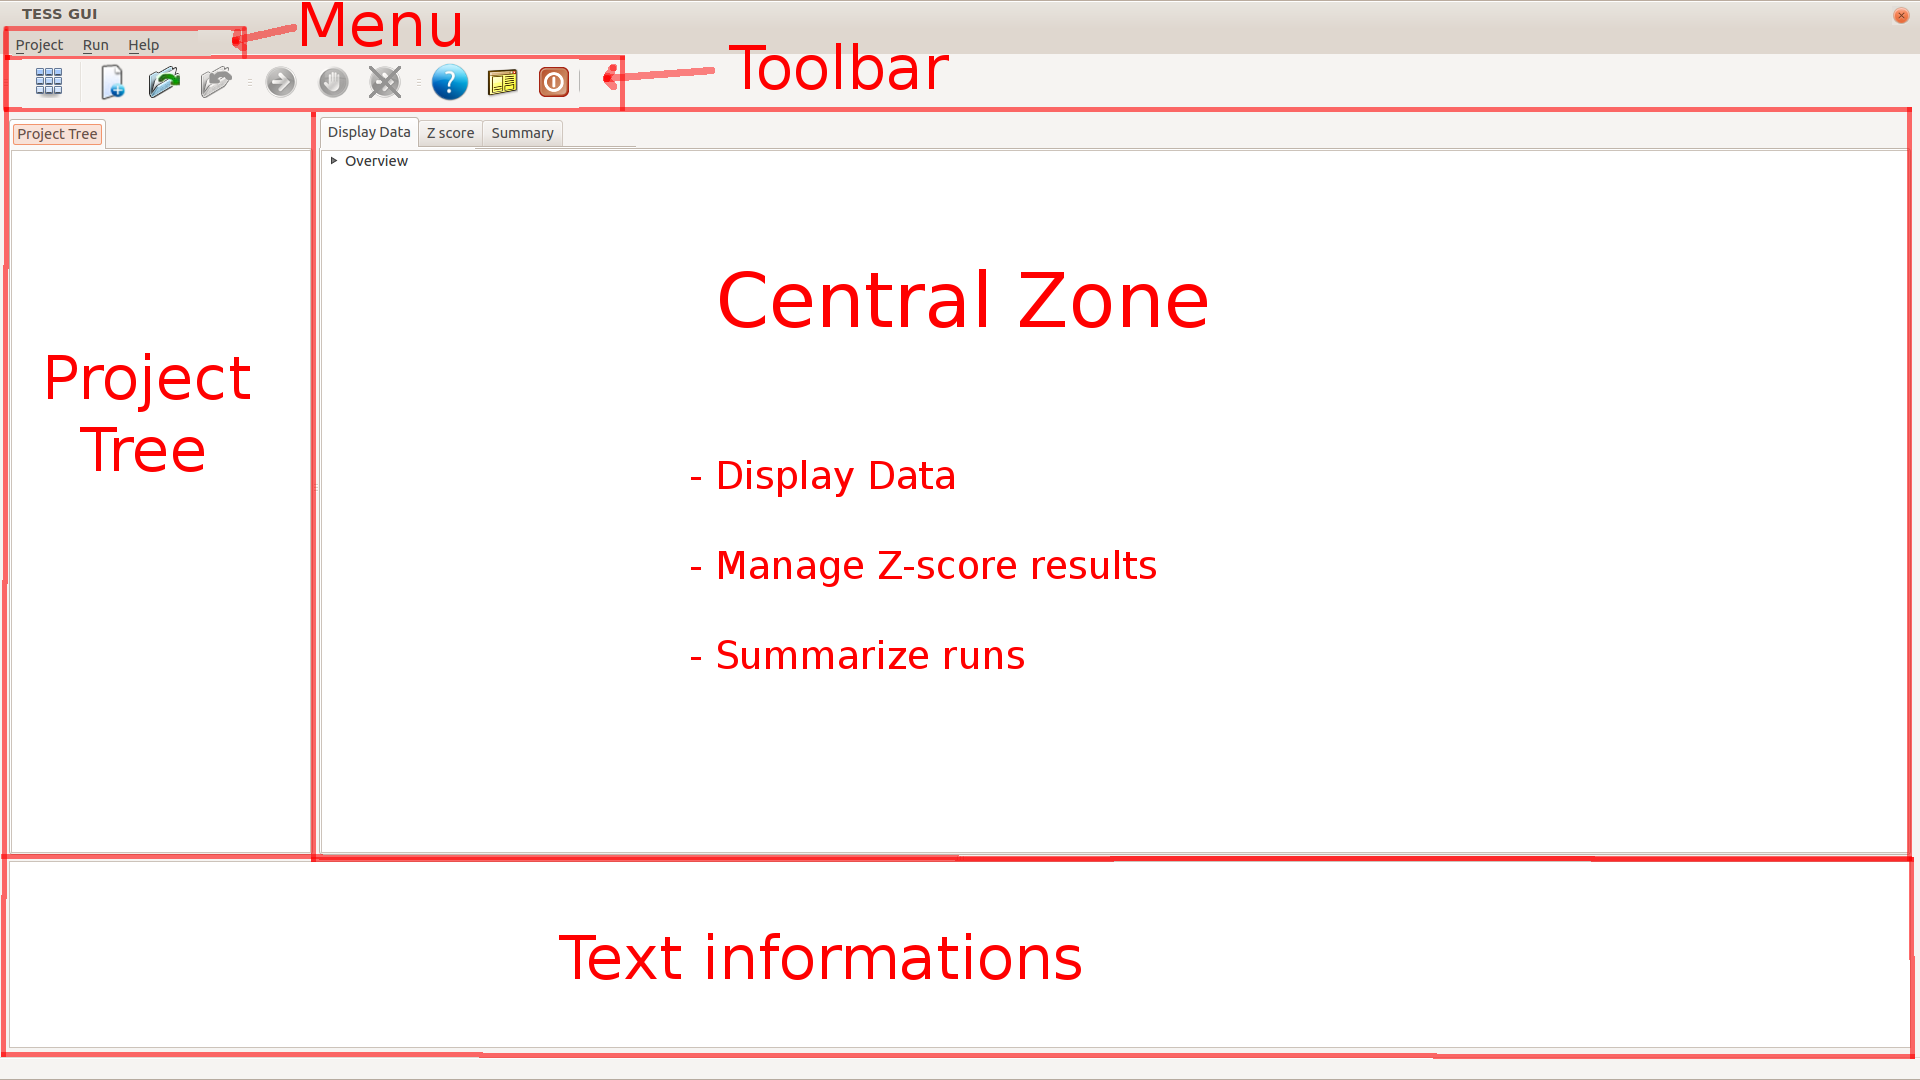
\includegraphics[width=17cm]{images/mainwindow2.png}
\caption{Main Window}
\end{figure}

The following parts describe each part of LFMM GUI. 

\subsubsection{The Menu}
\begin{figure}[H]
\centering

\includegraphics[width=8cm]{images/menu.png}
\caption{Menu description}
\end{figure}
The menu contains a set of possible actions. These actions are organized in 3 groups:
\begin{itemize}
\item a Project manager: to create, open, save, and close projects, 
		 	and to open textual results,
\item a Run manager: to set, abort and remove runs,
\item a Menu.
\end{itemize}

\subsubsection{The Toolbar}
\begin{figure}[H]
\centering

\includegraphics[width=12cm]{images/toolbar.png}
\caption{Toolbar description}
\end{figure}
The toolbar contains the same set of possible actions as the menu. Here is a description of the action
associated with each button:
\begin{itemize}
\item 
\includegraphics[width=0.6cm]{images/filedata.png} opens any data file,
\item 
\includegraphics[width=0.6cm]{images/filenew.png} starts a new project,
\item 
\includegraphics[width=0.6cm]{images/fileopen.png} opens an existing project,
\item 
\includegraphics[width=0.6cm]{images/fileclose.png} closes the current project (It is not mandatory to 
close the current project to open or create a project),
\item 
\includegraphics[width=0.6cm]{images/filequit.png} saves the current project and closes the GUI,
\item 
\includegraphics[width=0.6cm]{images/projectrun.png} starts a new run, 
\item 
\includegraphics[width=0.6cm]{images/projectabort.png} aborts the current run, 
\item 
\includegraphics[width=0.6cm]{images/removerun.png} removes a run from the current project (To do it, just select in the browse panel, the directory to remove), 
\item 
\includegraphics[width=0.6cm]{images/helpreference.png} displays the reference manual, 
\item 
\includegraphics[width=0.6cm]{images/helpabout.png} displays general information about LFMM GUI. 
\end{itemize}

\subsubsection{Textual Information}

The textual information displays all information printed by programs called by the GUI.
\begin{itemize}
\item it checks that input files were read correctly,
\item it informs you step-by-step of the execution of the current run,
\item it checks that a manhattan plot is correctly generated.
\end{itemize}
Please, if anything went wrong, check the textual information box to get more information.
\\
\noindent
{\it Tips:} When you start a run, the corresponding command line for the run is printed in the 
textual information panel.

\subsubsection{The project Tree}
\begin{figure}[H]
\centering
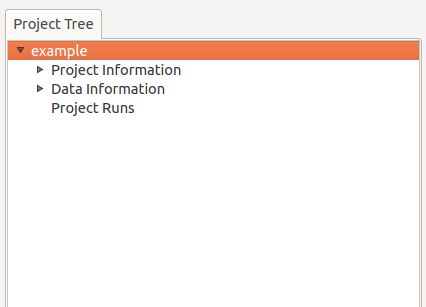
\includegraphics[width=8cm]{images/projecttree.png}
\caption{Project Tree global view}
\end{figure}
The project tree summarizes the current project information. 
As show in figure 4, the project tree information is grouped in 
\begin{itemize}
\item the project information: name of the project, date of creation, path to the project, the data
file in lfmm format, the data file in original format, the environmental file, and if provided, 
the SNP name file.
the data information, and information for each run.
\item the data information: number of individuals, and number of loci.
\item information for each run: algorithm, number of latent factors $K$, total number of sweeps, burn
in number of sweeps, and number of processes used, the textual result file, deviance criteria, and DIC
criteria.
\end{itemize}
{\it Tips 1: } To display a data file, you can double-click on it in the project tree. It is displayed in the "Display data" tab of the central zone.
\\
{\it Tips 2:} If you double-click on a textual result file, it loads this result 
file and displays it in the Z-score tab of the central zone.
\subsubsection{The Central Zone}

\begin{figure}[H]
\centering

\includegraphics[width=8cm]{images/tabs.png}
\caption{Tabs of central zone}
\end{figure}
The central zone is the main part of the GUI. As shown in figure 5, it is divided in 3 different panels (Display Data, Z-score, and summary). Each panel is described below.

\paragraph{Display Data}

This panel displays the data files. Each time you click on a data file in 
the Project Tree, the data is displayed here. 

\begin{figure}[H]
\centering
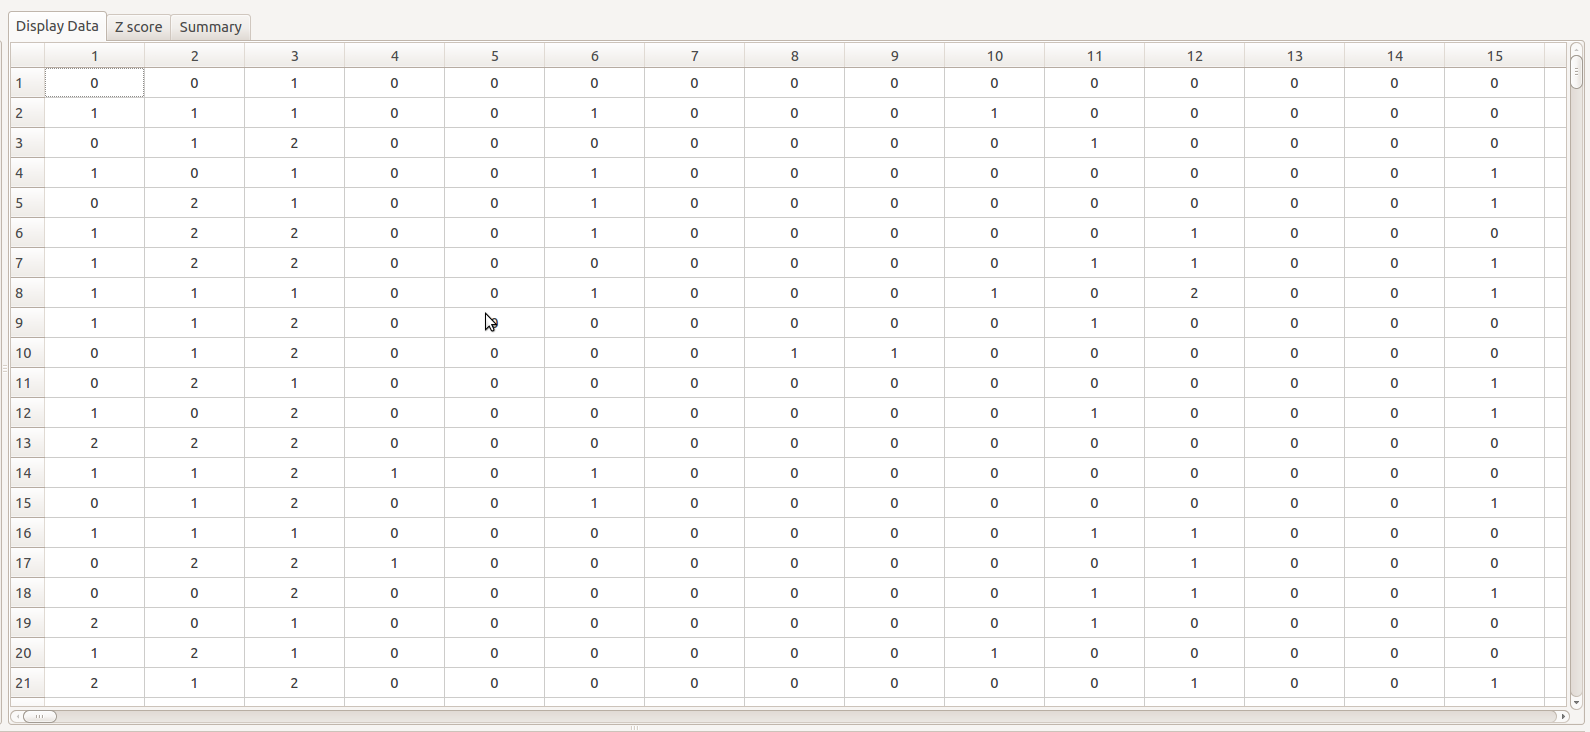
\includegraphics[width=16cm]{images/display_data.png}
\caption{Display data panel}
\end{figure}

\paragraph{Z-score}

\begin{figure}[H]
\centering
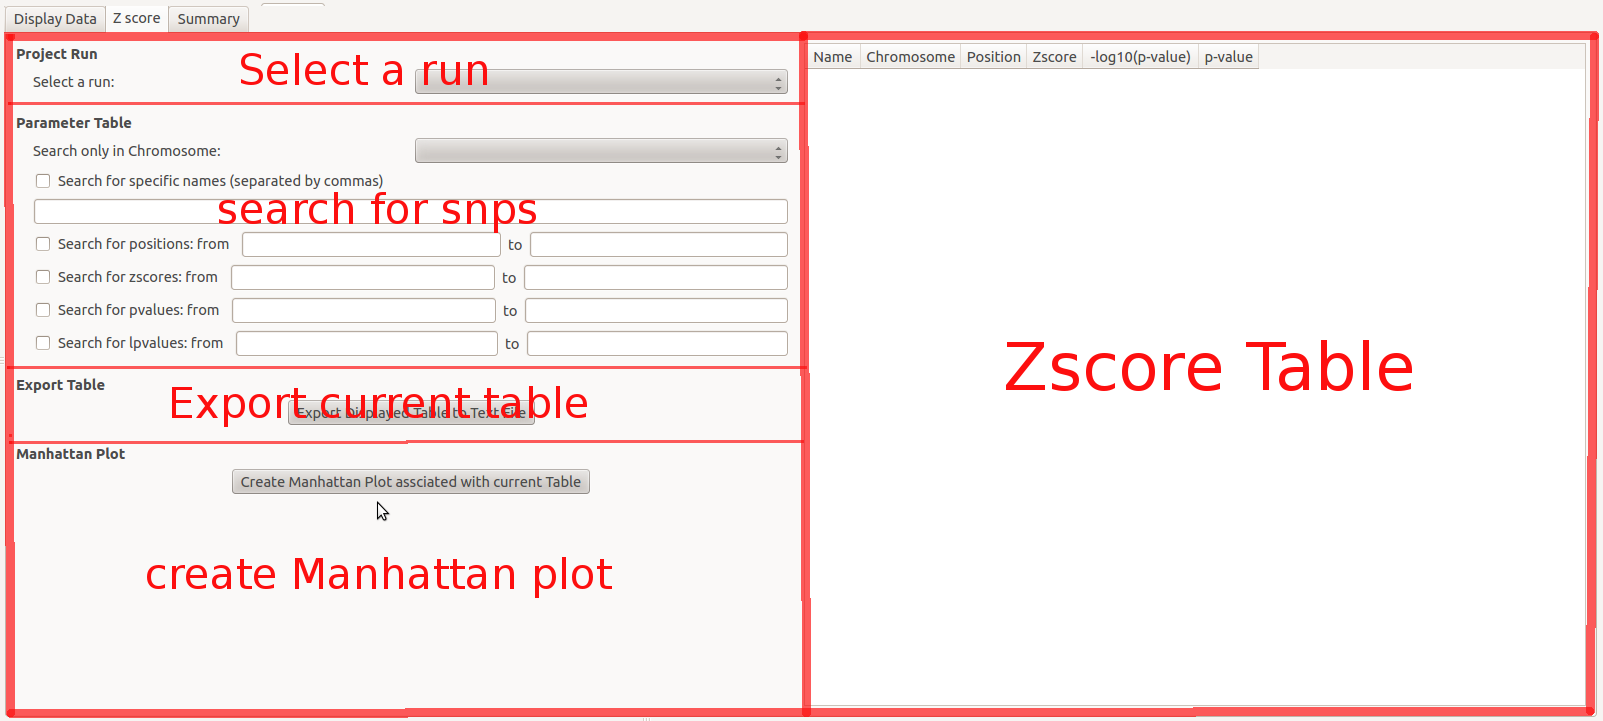
\includegraphics[width=16cm]{images/zscore2.png}
\caption{Z-score panel}
\end{figure}

Results can be analysed in the panel. As shown in figure 6, you can display
your results in a table. 
\\
{\it Tips:} If you did not provide a snp data file, SNPs are ordered in the same order
as they are given in the genotype data file. The $i^{th}$ SNP is called SNP\_$i$ at position $i$.
In this case, all SNPs are in chromosome $0$.
\\
With this tool, you can
\begin{itemize}
\item select the run of the project that you want to analyze. If you double-click on a specific zscore
file in the Project tree, it automatically shows the associated zscore table.
\item know the number of SNPs currently displayed in the table.
\item search for a specific snp or a group of SNPs in a single chromosome by selecting its names or 
a range of positions, zscores, pvalues, or $-log_{10}$(pvalue). You can select or unselect a criteria
by using the checkbox at the beginning of each criteria. For example, if want to select all SNPs in 
with a zscore upper than 3. You write 3 in the first bound box of zscore line and check the
corresponding checkbox. 
\item order them by name, Chromosome Position, Zscore, pvalue, and $-log_{10}(pvalue)$.
\item export the current displayed zscore table in a text file.
\item display the manhattan plot associated with the current zscore table. The manhattan plot is displayed with a R script in pdf. If the pdf is not displayed, you can probably find it in your directory of you project with the name "manhattan\_plot.pdf". If the pdf is displayed, we advise you to use your own pdf viewer to register it in a proper name and space. The upper button for manhattan plot displays a manhattan plot with only SNPs currently in the zscore table. For example, if you selected a
specific chromosome and a specific range of positions, it displays only these SNPs. The lower button
for manhattan plot displays all the SNPs and black and grey and it underlines in green those 
which are currently in the zscore table. For example, it can underline a manhattan of SNPs
(ie a group of SNPs in the same region with significant correlation).
\end{itemize}


\paragraph{Summary}

\begin{figure}[H]
\centering
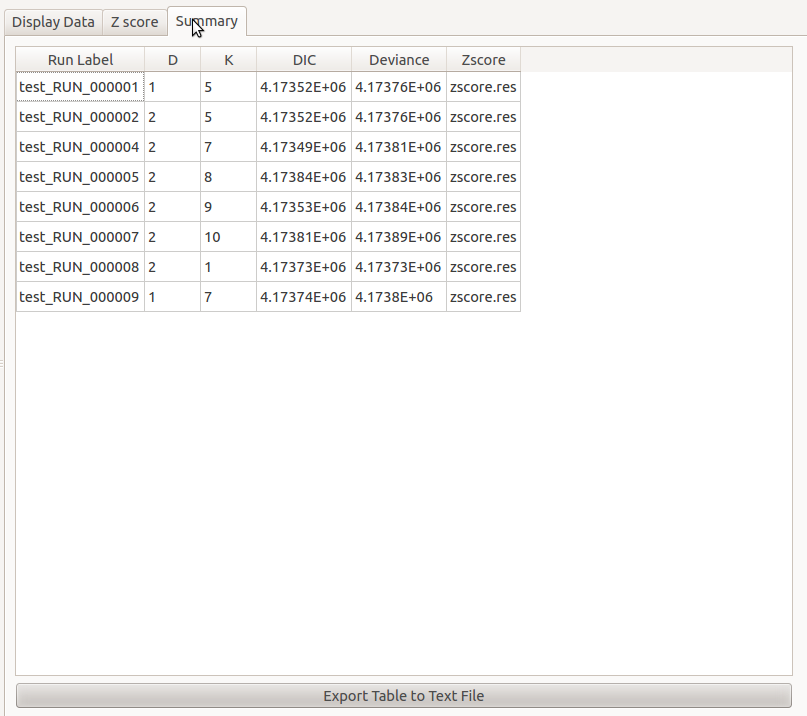
\includegraphics[width=16cm]{images/summary_panel.png}
\caption{Summary panel}
\end{figure}

This panel provides a global view of the runs. As shown in figure 8, it displays 
a summary table of the runs. In the table, you can find information about each run, such as the label, the variable used, the number of latent factors, the DIC criteria, the deviance criteria, and the name of the Zscore file. You can also export this table in text format. We advise you to be really
careful in the interpretation of DIC�criteria. For example, we do not advise you to use DIC criteria to 
select the number of latent factors $K$. 

\subsection{New Project}
When using the GUI shell, users work with projects. A project is a coherent unit
which groups the input data, the algorithmic parameter settings, and the output results
altogether. To create a new project, access the menu "Project=New Project..." or the 
corresponding button on the tool bar (see Figure 3). The GUI shell shows the "New
Project" dialog box (see Figure 9).

\begin{figure}[H]
\centering
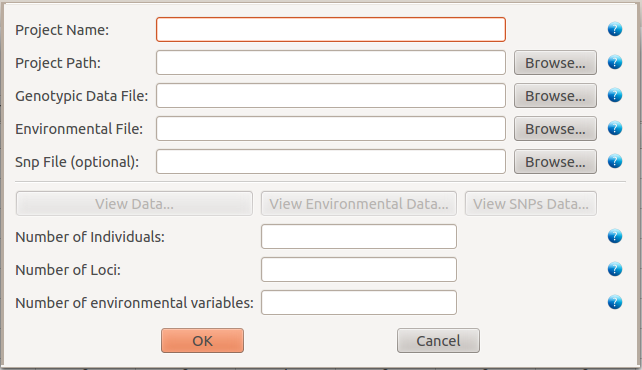
\includegraphics[width=8cm]{images/newproject.png}
\caption{new project}
\end{figure}

The user should name his/her project and choose the project path and data (tip:
using the "Browse..." is a convenient way to input this information). Note that LFMM
requests its user to put his/her data in the same directory of the project file itself. We also
recommend users to store different projects using separate directories for clear organization
of information, although LFMM does not require this.

The user also needs to input the number of individuals, number of loci 
and number of environmental variables.
He/she can also enter a snp data file. This file is optional. 
If the user is not clear of this information, he/she can always click the "View Data..."
button to check the data first (see Figure 9). 
Users should input information and the format of the data with care. 
Although the software can catch most common errors, wrong inputs may result in strange analytical
results.
\\
\noindent
{\it Tips:} If you did not provide a snp data file, SNPs are ordered in the same order
as they are given in the genotype data file. The $i^{th}$ SNP is called SNP\_$i$ at position $i$.
In this case, all SNPs are in chromosome $0$.
\\

When inputs are finished, click on the "OK" button to confirm the creation of the new project.
When the project is created, the GUI shell checks that all requirements are followed. 
Then, it converts the data file in lfmm format, automatically load it, and show its
data to the user. If the dataset is a bit large (more than 5000 SNPs), the conversion in lfmm 
format can take a few minutes.

\subsection{New Run}

\begin{figure}[H]
\centering
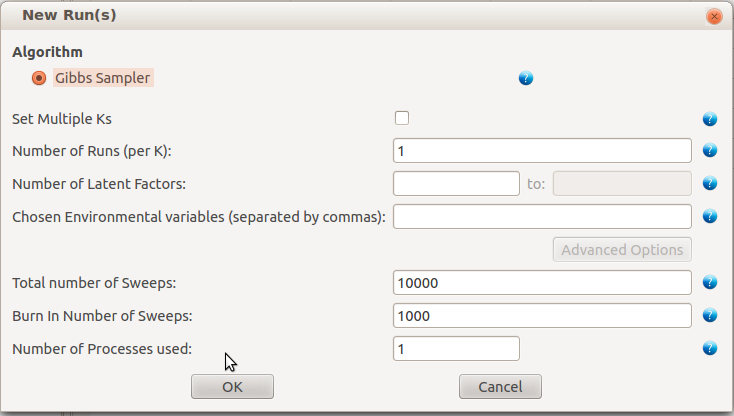
\includegraphics[width=8cm]{images/newrun.png}
\caption{New run box}
\end{figure}
The user can then start a run by accessing the menu
"Project=Run..." or the corresponding button on the tool bar (see Figure 3). The GUI shell shows
the "New Run(s)" dialog box asking the user to key in the required run information (see
Figure 9).
This box allows users to choose 
\begin{itemize}
\item the algorithm
\item the number of latent factors that you want to use. You can launch several runs at the same time
with the same value of $K$ or different values of $K$.
\item a list of environmental variable number. A run is launched sequentially for each
environmental variable number listed (Ex: 1,2,5. A run is launched for the first, the second
and the fifth environmental variable).
\item the total and burn in number of sweeps.
\item the number of processes. Choosing several processes multithreads the 
algorithm and by consequence speed up the runs. The result is the same with one or several 
processes. To ensure the algorithm to be speeded up, we advise you to choose the number of processes 
at most equal to the number of processes of your computer.

\end{itemize}

\section{An example/Tutorial}
\noindent
All examples are available in the directory example. The goal of this tutorial is to 
introduce the potential of this software. 

\subsection{Data Set}

The data set that we analyze in this tutorial is an Asian human data set of SNPs data.
This data is a worldwide sample of genomic DNA (10757 SNPs) from 388 individuals,
taken from the Harvard Human Genome Diversity Project - Centre
Etude Polymorphism Humain (Harvard HGDP-CEPH)2 . In those
data, each marker has been ascertained in samples of Mongolian 
ancestry (referenced population HGDP01224) \cite{Patterson_2012}. We selected all 
samples from Asia. Using Tracy-Widom tests implemented in {\tt SmartPCA}  
\cite{Patterson_2006}, we found that the number of
principal components with P-values smaller than $0.01$ was around $KTW = 10$. Using
the Bayesian clustering programs {\tt STRUCTURE} \cite{Pritchard_2000} and {\tt TESS}
\cite{Chen_2007, Durand_2009}, we found that $K = 7$ 
components could better describe our simulated data.
We extracted climatic data population samples using the WorldClim 
data set at 30 arcsecond (1km2 ) resolution 
(Hijmans, Cameron, Parra, Jones, and Jarvis (2005)).
We summarized the climatic variables by using the first axis of a 
principal component analysis for temperature variables and for 
precipitation variables. 
The data set is in directory \verb|examples/human_example/|. The genotype information
are in \verb|panel11_Asia.lfmm|. the SNPs information is in \verb|panel11.pedsnp|. 
The environmental file is \verb|cov_panel11_Asia.env|. There are 2 variables, one proxy
for temperature and one for precipitation. 


\subsection{Launch LFMM}
Let us start to analyze this data. The first step is to install LFMM. You can find all 
explanations in the section Installation of the documentation. Once it is installed, you 
can run LFMM GUI by clicking on the created executable. You can recognize the menu and 
the toolbar at the top, the project tree on the left, the text information box at the 
bottom, and the central zone.

\subsection{New project}
To analyze our dataset, we create a new project. You can click on the 
new project button in the toolbar:
\begin{center}

\includegraphics[width=1.5cm]{images/filenew.png}
\end{center}
A new box is displayed. It asks you some information to start your project. We fill it in
as show in the following figure.
\begin{center}
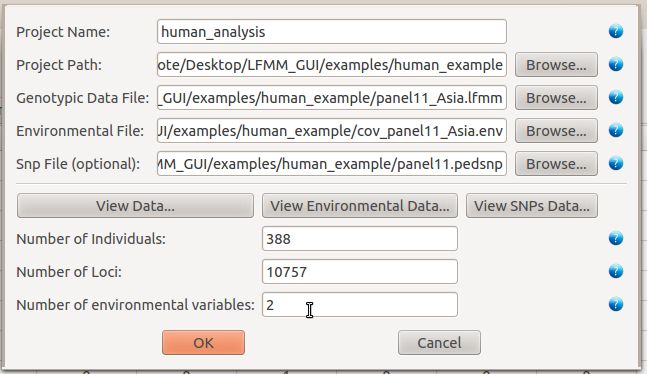
\includegraphics[width=8cm]{images/newproject_Asia.png}
\end{center}

The name of the data project is \verb|human_analysis|. The project directory is 
\verb|human_example|. Each time that you need to fill a directory or an existing file,
you should fill the entire path to it. That is why we advise you to use the "Browse"
button. This directory should contain the data set to analyze.
The genotype data set is \verb|panel11_Asia.lfmm|. The environmental file is 
\verb|cov_panel11_Asia.env|. The snp file is \verb|panel11.pedsnp|.
You can use the "view" buttons to have a preview of these files. For the genotype file,
it can be a bit slow. The number of individuals is 388. The number of loci is 10757. 
The number of environmental variables is 2.
\\
\noindent
{\it Tips:} If you have forgotten what a field should contain, you can click on the interogation
point buttons. 

We are ready to create this new project. You can click on "OK". The software checks
the consistency of your information and create the new project. If anything goes wrong,
the detected inconsistency is displayed in a warning message.
The genotype data information is displayed in the central zone and the project tree is filled with information
you provided. you can click on the elements of the project tree to see them. 
In the project tree, you can click on any file to obtain its preview.
\begin{center}
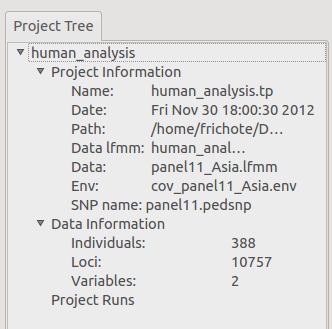
\includegraphics[width=6cm]{images/projecttree_Asia.png}
\end{center}


\subsection{New Runs}
Now that we have created a project, we can analyze our data and launch LFMM.
To start it, you can click on the new run button in the toolbar:
\begin{center}

\includegraphics[width=1.5cm]{images/projectrun.png}
\end{center}

A new box pops up. It asks you some information to start your project. We fill it
as show in the following figure.
\begin{center}
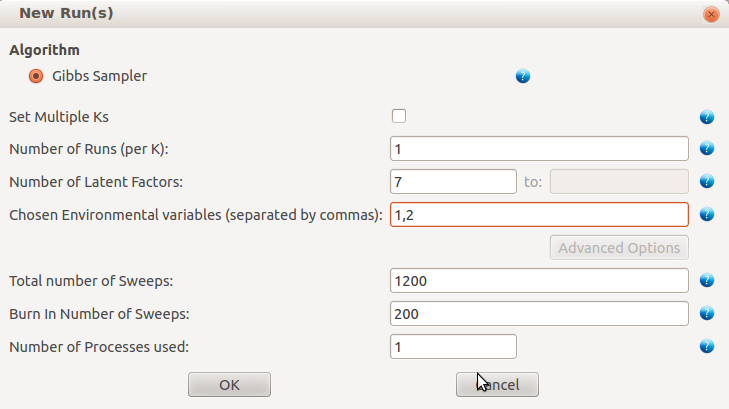
\includegraphics[width=12cm]{images/newrun_Asia.png}
\end{center}
We set one run per value of $K$, the number of latent factors. We 
choose to set $K=7$ because it was the result returned by {\tt TESS} and {\tt STRUCTURE}.
Several value should be tested. As we want to launch LFMM with the environmental 
variable 1, the temperature and then the environmental variable 2, the precipitation, we set
the environmental variable to "1, 2". We set a total number of sweeps to 1200 and a burnin number
of sweeps to 200. These values should be carefully chosen. It is dependent of the size of your
data set for example. As we don't know the capacity of your computer, we set the number of 
processes to 1.
We are ready to launch the runs. You can click on "OK". The software checks
the consistency of your information and launch the first run. If anything goes wrong,
a warning message indicates the detected inconsistency.
Information about the stat of the current run is displayed in the information
box at the bottom. On this data set, a run should be of a few minutes at most. On my laptop,
it takes around 7 minutes per run with one process. So, you can
get a cup of cofee or tea.
You also notice that this new button appeared:
\begin{center}

\includegraphics[width=1.5cm]{images/projectabort.png}
\end{center}
You can click on it if you want to abort the runs that you launched.

\subsection{Analyze Run}
Both runs that you launched should be over. When a run is over, the results are automatically
displayed in the Zscore panel, as follows:
\begin{center}
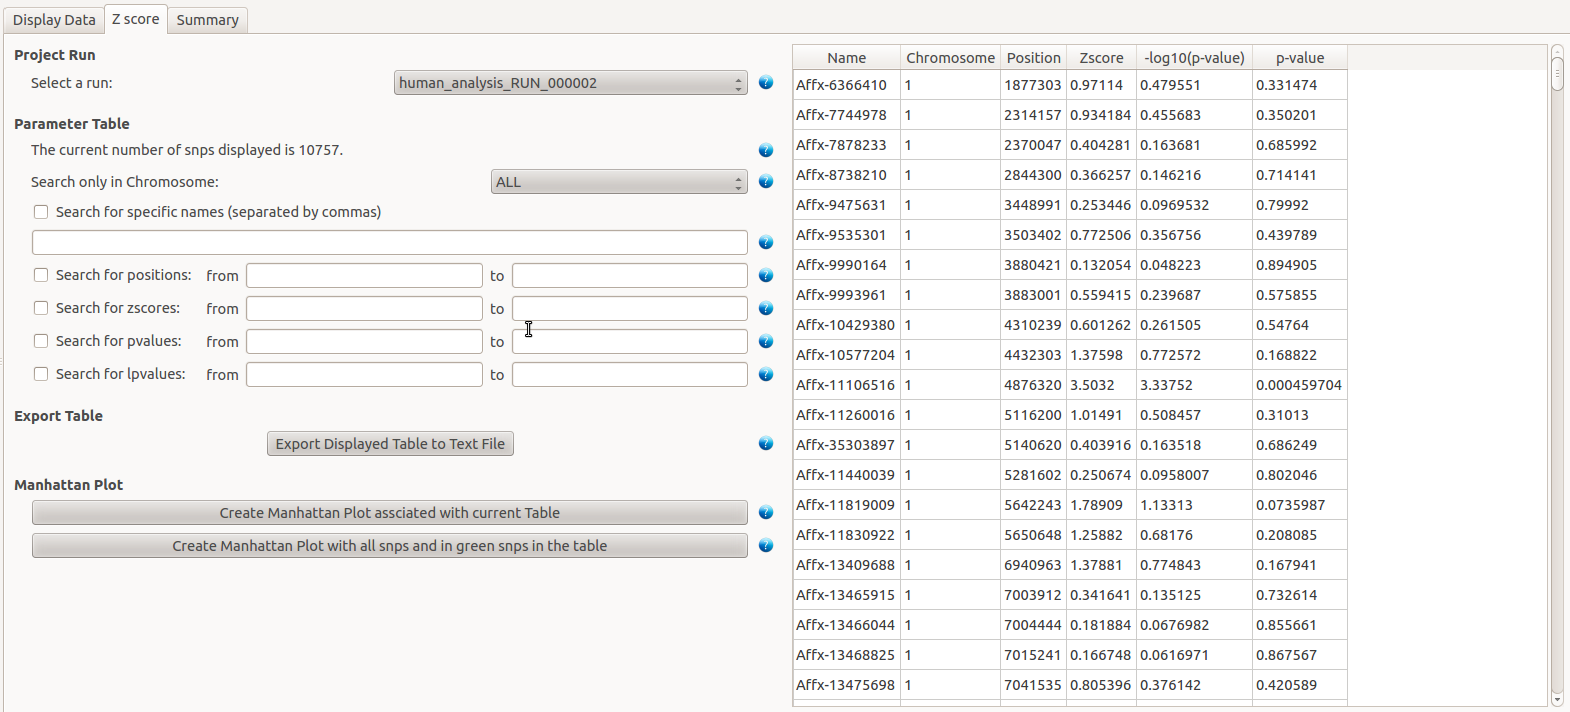
\includegraphics[width=16cm]{images/zscore_Asia.png}
\end{center}

The results can be analyzed. As you can see, in the table at 
the right of the Zscore panel, the SNPs are displayed with their information and their results.
For example, we analyze results for environmental variable 2. We select at the top, 
\verb|human_analysis_run_2|. 
\begin{center}

\includegraphics[width=13cm]{images/selectrun.png}
\end{center}
If you do not remember which run used variable 2, you can check it
in the summary table panel.
\begin{center}
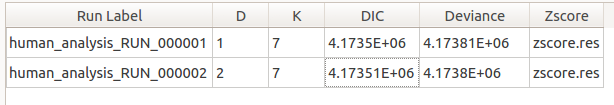
\includegraphics[width=13cm]{images/summary_Asia.png}
\end{center}
We can create a global manhattan plot to have a visual idea of the results.
Just click on the button, "create Manhattan plot associated with the current table".
A manhattan plot, similar to the one below is displayed:
\begin{center}
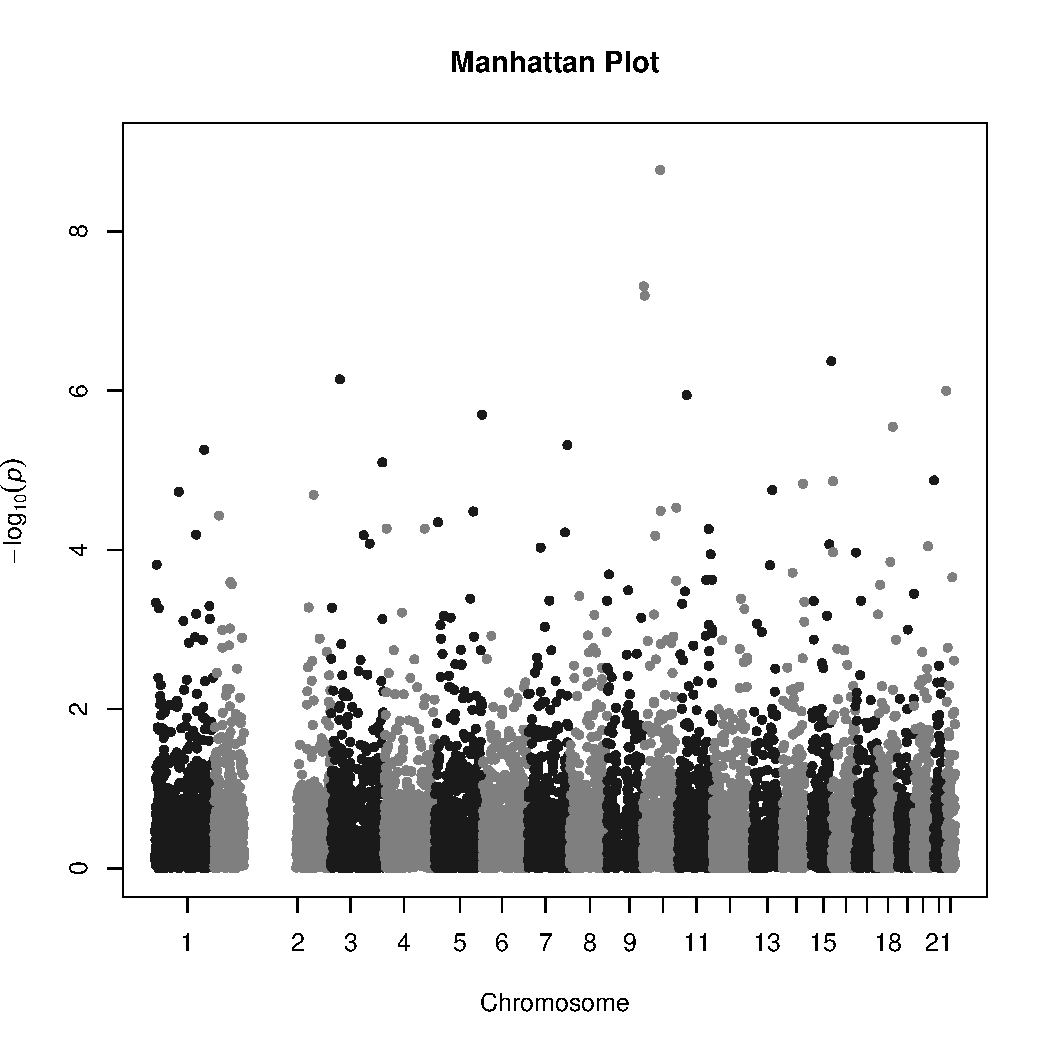
\includegraphics[width=12cm]{images/manhattan_plot.pdf}
\end{center}
We can observe that some SNPs are significantly associated with this variable 2 because they
have a high $-log_{10}(P-value)$. 
More precisely, for example, we would like to have a list of SNPs with $-log_{10}(P-value)$ 
higher than 4. To do this, we just have to fill the range for the corresponding box and check
the checkbox as follows:
\begin{center}

\includegraphics[width=15cm]{images/lpvalue_Asia.png}
\end{center}
The number of SNPs is displayed as follows:
\begin{center}

\includegraphics[width=11cm]{images/nb_lpvalue_Asia.png}
\end{center}
Another example could be that we would like to analyze SNPs in chromosome 10. To do this, we 
just have to select chr10 in the list as follows:
\begin{center}
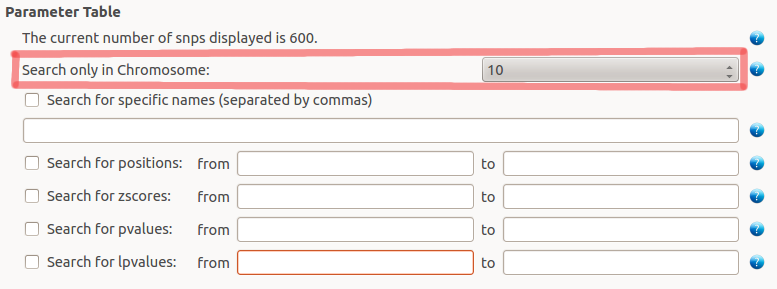
\includegraphics[width=13cm]{images/chr10_Asia.png}
\end{center}
We can also display the manhattan plot for this specific chromosome by clicking on the button
"create Manhattan plot associated with the current table" after we selected chromosome 10.
A manhattan plot, similar to the one below is displayed:
\begin{center}
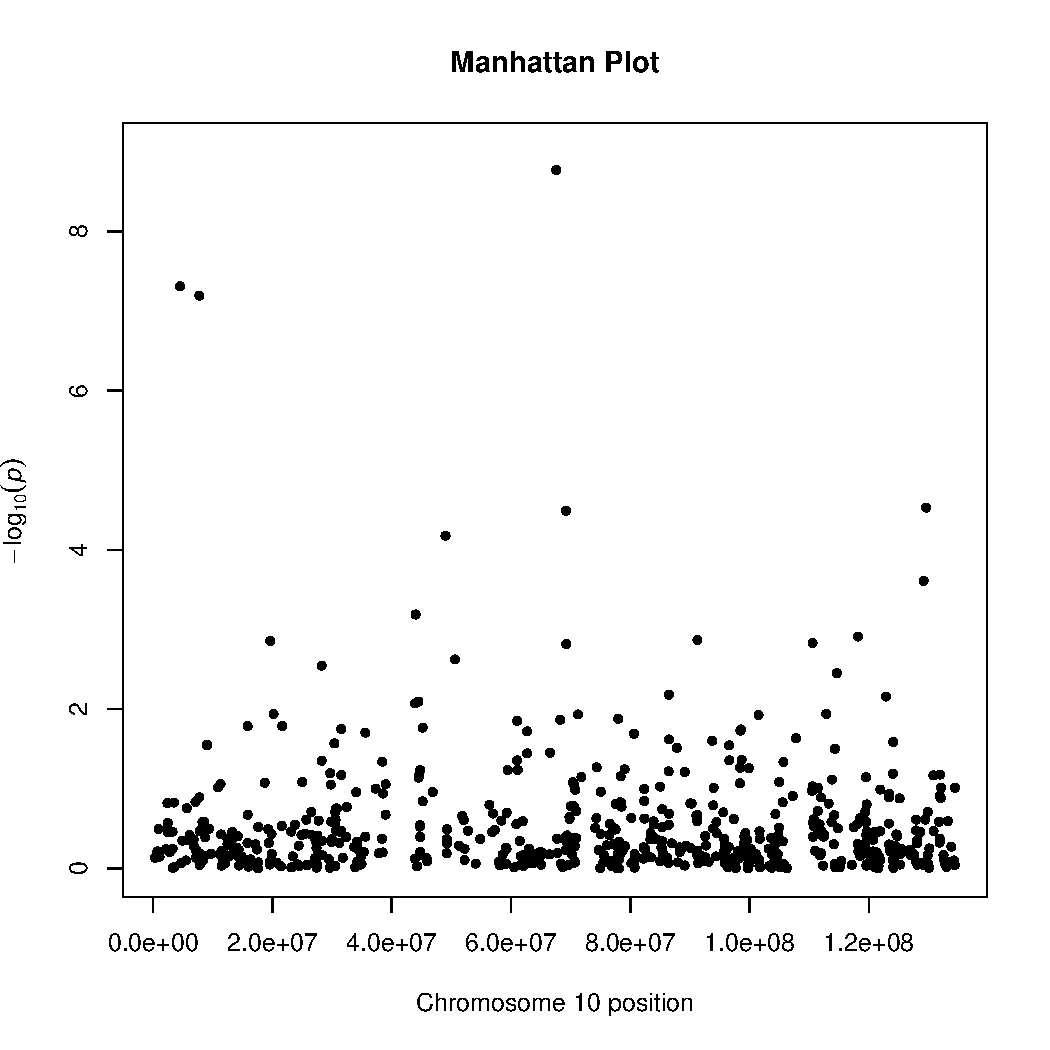
\includegraphics[width=12cm]{images/manhattan_plot_chr10.pdf}
\end{center}
Finally, for example, we would like to know if SNPs Affx-3561055 and Affx-3582668 are 
significantly correlated with variable 2. We can look for these SNPs by filling these 
names as follows:
\begin{center}
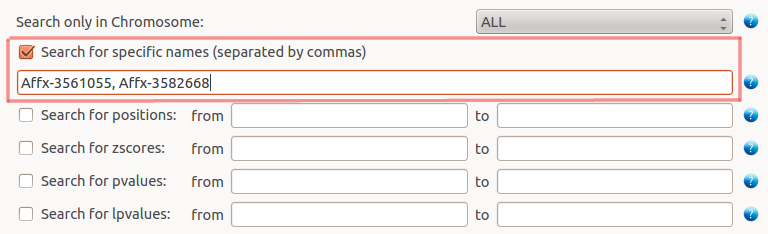
\includegraphics[width=13cm]{images/name_Asia.png}
\end{center}
We can also display the manhattan plot with all SNPs and these two SNPs underlined in green by clicking 
on the button "create Manhattan plot with all SNPs and in green SNPs in the table table" after 
we looked for these SNPs in the zscore table.
A manhattan plot, similar to the one below is displayed:
\begin{center}
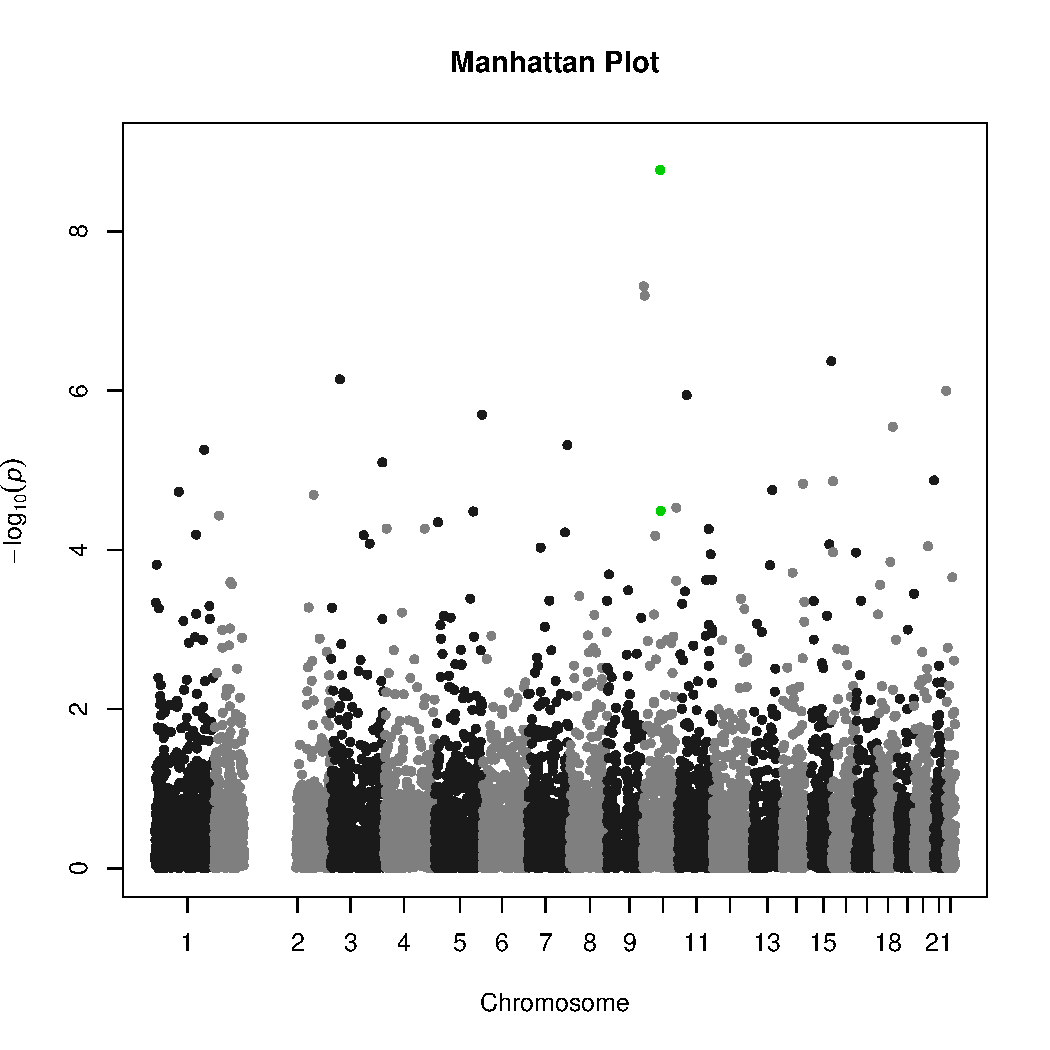
\includegraphics[width=12cm]{images/manhattan_plot_green.pdf}
\end{center}

\bibliography{biblio}
\bibliographystyle{plain}

%\bibliography{manuscript}
%\bibliographystyle{apalike}

\end{document}

   
